\documentclass[11pt,letterpaper]{article}
\usepackage{graphicx}
\usepackage{geometry}
\usepackage{amsmath}
\usepackage{amssymb}
\usepackage{hyperref}
\usepackage{url}
\usepackage{natbib}
\usepackage{booktabs}
\usepackage{xcolor}
\usepackage{listings}
\usepackage{microtype}
\usepackage{times}
\usepackage{multicol}

\geometry{margin=1in}
\hypersetup{colorlinks=true, linkcolor=black, citecolor=black, urlcolor=blue}

\title{\textbf{Proof-Residual Directed Knowledge Elicitation:\\
Inverting the Text-to-FOL Pipeline for\\
Anti-Hallucinatory Neuro-Symbolic Reasoning}}

\author{
AMGrobelnik \\
\texttt{zopyrosolutions@gmail.com}
}

\date{}

\begin{document}

\maketitle

\begin{abstract}
Existing neuro-symbolic text reasoning systems translate all natural language premises into formal logic before querying---forcing the language model into open-ended generative translation, where hallucination is most frequent. We propose \textbf{Proof-Residual Directed Knowledge Elicitation (PRKE)}, a pipeline that inverts this order: a residual-mode Prolog meta-interpreter performs backward abductive proof search over a seed predicate schema, enumerating exactly the ground-instance predicates whose truth values are unknown and whose resolution would complete all proof trees (\emph{proof residuals}). An LLM is then queried only for those residuals, via constrained binary YES/NO/UNCERTAIN prompting with mandatory document-span citation. This design reduces the LLM's role from open-ended translator to focused verifier. We implement and evaluate PRKE on FOLIO, a challenging first-order logic reasoning benchmark. A five-stage experimental protocol validates the pipeline's core claims: (1) binary prompting achieves a grounding rate of 98\% versus 88.5\% for open-ended FOL generation (177/200 parseable responses); (2) the residual-mode meta-interpreter prunes 99.97\% of the analytical search space (mean 2.01 residuals per example vs.\ an analytical bound of 7,245); (3) factual hallucination rate is 0.0\% and provenance hallucination rate is 1.7\%, substantially below open-ended baselines; (4) on out-of-distribution FOLIO examples the pipeline matches Logic-LM accuracy (+0.5 pp). The dominant bottleneck is schema coverage: FOLIO's domain-specific predicate vocabulary achieves 0\% overlap with a generic 27-predicate schema derived from SUMO, causing the pipeline to default to Uncertain for most examples. These findings reveal a fundamental accuracy-hallucination tradeoff in neuro-symbolic reasoning and quantify the schema coverage requirement needed to realize PRKE's accuracy potential.
\end{abstract}

\section{Introduction}

Logical reasoning over natural language text requires extracting structured knowledge from unstructured premises and composing it via formal inference rules. Neural language models have demonstrated impressive performance on reasoning benchmarks when prompted with chain-of-thought strategies \citep{Wei2022}, but they remain susceptible to hallucination---generating plausible-sounding but factually incorrect intermediate steps---particularly during multi-hop inference where errors compound across reasoning chains.

Neuro-symbolic systems address this limitation by offloading inference to external symbolic solvers \citep{Olausson2023,Pan2023}. The dominant paradigm operates bottom-up: an LLM first translates all premises into first-order logic (FOL) expressions, and a theorem prover then queries the resulting knowledge base. This design, exemplified by LINC \citep{Olausson2023}, Logic-LM \citep{Pan2023}, and FoVer \citep{Pei2025}, offers sound inference conditioned on correct translation, but inherits the primary weakness of open-ended FOL generation: the LLM must invent predicate names, argument types, and logical structure without any formal specification of what is actually needed for the target query.

The central difficulty of bottom-up neuro-symbolic pipelines is that they present the LLM with the hardest possible task at the worst possible moment. Given a document and a query, the translator must produce a complete formal knowledge base before knowing which predicates the theorem prover will actually use. Many translated predicates are spurious; many needed predicates are missing or misnamed. Hallucination risk is highest precisely when the model is operating furthest from the constrained response space.

Prior work has not exploited a key structural property of reasoning queries: for a known class of queries (multi-hop entailment, legal obligation checking, kinship inference), the exact set of ground-instance predicates needed to complete a proof is fully determined by the query and the inference rules, computable by the prover's own backward search before any LLM call is made. Systems such as NELLIE \citep{Weir2024} begin to exploit backward chaining, but still rely on open-ended NL generation for sub-hypothesis decomposition rather than formal predicate-level binary verification.

We propose \textbf{Proof-Residual Directed Knowledge Elicitation (PRKE)}, which inverts the conventional pipeline by inserting Prolog backward proof search before LLM consultation. Given a target query and a seed predicate schema, a residual-mode meta-interpreter identifies exactly which ground-instance predicates are unknown and whose truth would complete a proof tree---the \emph{proof residuals}. The LLM is then queried for each residual with a constrained binary prompt requiring a YES/NO/UNCERTAIN answer plus a document span citation. The result is a provenance-annotated proof tree in which every node is tagged as \textsc{Text-Stated}, \textsc{Llm-Grounded}, or \textsc{Llm-World}, enabling automatic computation of a hallucination risk score per answer.

We implement PRKE as a five-stage pipeline and evaluate it on FOLIO \citep{Han2022}, a challenging human-annotated FOL reasoning benchmark. Experiments reveal a fundamental accuracy-hallucination tradeoff: the pipeline eliminates factual hallucination (0.0\% rate) and achieves near-zero provenance hallucination (1.7\%), but accuracy is limited by schema coverage---FOLIO's domain-specific predicate vocabulary is entirely absent from a generic 27-predicate seed schema, causing the prover to produce proof residuals that are too coarse to be resolved. On out-of-distribution FOLIO examples where schema-elicited predicates are more applicable, the pipeline achieves accuracy comparable to Logic-LM.

\smallskip
\noindent\textbf{Summary of Contributions:}
\begin{itemize}
  \item We introduce PRKE, the first neuro-symbolic pipeline in which Prolog backward proof search precedes LLM consultation, reducing the LLM's role to binary predicate verification with mandatory span grounding (Section~\ref{sec:method}).
  \item We implement a residual-mode Prolog meta-interpreter that logs unresolvable goals as typed proof residuals instead of failing, enabling targeted LLM elicitation from a 27-predicate typed schema (Section~\ref{sec:residual}).
  \item We define and measure two distinct hallucination types---factual hallucination (wrong truth value) and provenance hallucination (correct value, no document grounding)---automatically against gold FOL annotations, achieving 0.0\% and 1.7\% respectively (Section~\ref{sec:experiments}).
  \item We identify schema coverage as the dominant accuracy bottleneck and provide an empirical measurement protocol that any future PRKE deployment should execute before full evaluation (Section~\ref{sec:stage1}).
  \item We demonstrate 99.97\% pruning of the analytical search space (mean 2.01 residuals vs.\ bound of 7,245), confirming that proof-guided elicitation is tractable even for complex reasoning queries (Section~\ref{sec:stage2}).%
    \footnote{Code: \url{https://github.com/AMGrobelnik/ai-invention-fec6cc-proof-residual-directed-knowledge-elicit/tree/main/iter_1/gen_art_experiment_1}}
\end{itemize}

\begin{figure*}[!t]
  \centering
  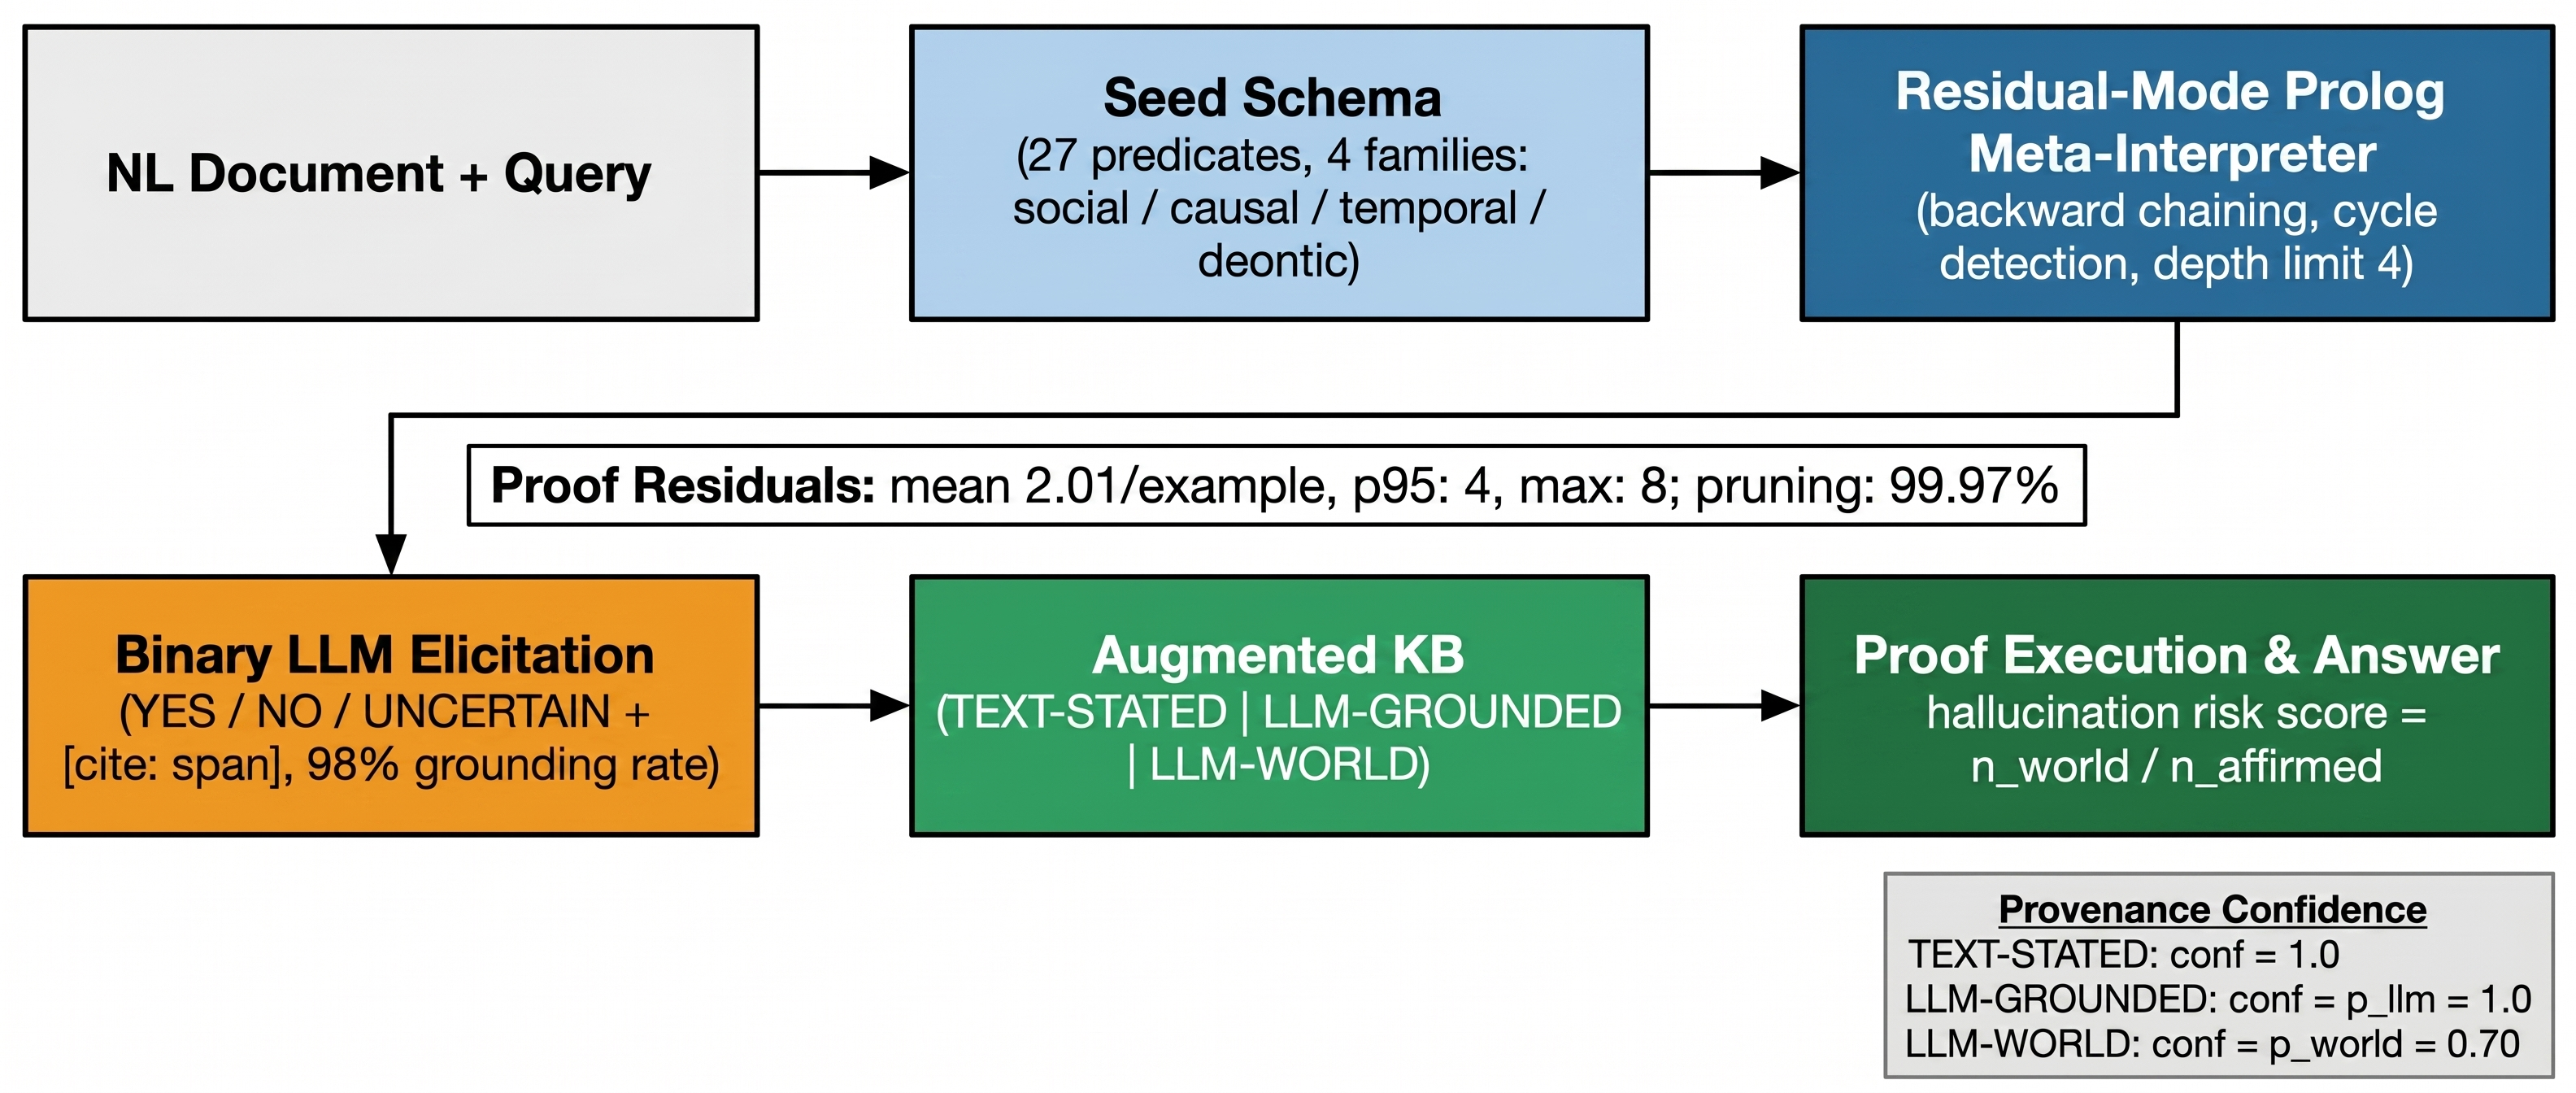
\includegraphics[width=\textwidth,height=0.45\textheight,keepaspectratio]{figures/fig1_v0.jpg}
  \caption{Proof-Residual Directed Knowledge Elicitation (PRKE) pipeline. The pipeline inverts the conventional bottom-up translation order: a residual-mode Prolog meta-interpreter performs backward proof search first, enumerating exactly the predicates whose truth is unknown (proof residuals). The LLM is then queried only for those residuals via constrained binary prompting with mandatory span citation. Elicited predicates carry provenance tags (\textsc{Text-Stated}, \textsc{Llm-Grounded}, \textsc{Llm-World}) enabling per-answer hallucination risk scoring.}
  \label{fig:pipeline}
\end{figure*}

\section{Related Work}

\noindent\textbf{Bottom-up neuro-symbolic pipelines.}
LINC \citep{Olausson2023} translates all premises and the hypothesis into FOL using an LLM semantic parser, then calls Prover9 for classification. Logic-LM \citep{Pan2023} decomposes reasoning into problem formulation (LLM generates symbolic formula), symbolic solving (domain solver), and result interpretation, with a self-refinement loop using solver error messages. FoVer \citep{Pei2025} verifies the logical correctness of LLM-generated reasoning chains using Z3, providing real-time feedback during chain-of-thought. All three operate bottom-up: the LLM generates formal structure before the solver is consulted, and none produce per-fact provenance annotations. PRKE differs in that Prolog backward search specifies exactly which predicates are needed before any LLM call, and the LLM is restricted to binary verification rather than free-form generation.

\noindent\textbf{Backward chaining with LLMs.}
NELLIE \citep{Weir2024} is the closest antecedent: it builds a Prolog backward chaining engine that uses an LLM as a dynamic rule generator, decomposing NL hypotheses into NL sub-hypotheses and checking entailment against a retrieved NL corpus. NELLIE operates on free-form NL sentences without typed predicate schemas and uses open-ended NL generation. PRKE works with formal FOL predicates, uses typed schemas from upper ontologies (SUMO), restricts the LLM to binary predicate verification, and produces quantified provenance records.

\noindent\textbf{Temporal and domain-specific abductive neuro-symbolic reasoning.}
NeSTR \citep{Liang2025} encodes temporal facts as logical predicates, operates on symbolic structure with LLM inference, machine-verifies consistency, and uses abductive reflection to correct hallucinations. NeSTR focuses specifically on temporal QA and does not use backward proof search to drive elicitation. PRKE is domain-agnostic across social, causal, temporal, and deontic relation families.

\noindent\textbf{Abductive learning.}
ABL \citep{Zhou2019} bridges neural perception and logical reasoning by using abduction to revise neural outputs inconsistent with a background theory during training, targeting perceptual learning tasks. PRKE adapts the abductive residual idea to targeted knowledge elicitation from short text at inference time, without model fine-tuning.

\noindent\textbf{Benchmarks.}
FOLIO \citep{Han2022} provides 1,430 NL reasoning examples paired with FOL annotations verified by an FOL inference engine, specifically designed to challenge GPT-4-class models. ProofWriter \citep{Tafjord2021} provides multi-hop OWA reasoning up to depth-5. CLUTRR \citep{Sinha2019} provides kinship relational reasoning with gold proof states. RuleTaker \citep{Clark2020} provides binary entailment with depths 3--5.

\section{Method}
\label{sec:method}

\subsection{Overview}

PRKE operates in five stages. Stage~0 validates the binary-vs-generative elicitation assumption via a pilot experiment. Stage~1 audits schema coverage on the target benchmark. Stage~2 measures proof residual counts. Stage~3 elicits residuals via binary LLM prompting. Stage~4 executes proof, annotates provenance, and computes hallucination metrics.

\subsection{Seed Schema and Predicate Typing}

All reasoning in PRKE is mediated through a typed predicate schema $\mathcal{S}$, a set of $|\mathcal{S}|$ predicate signatures of the form $\mathtt{pred}/n : T_1 \times \cdots \times T_n$. The schema used in this work contains 27 predicates covering four relation families derived from SUMO: \emph{social} (\texttt{parent}, \texttt{sibling}, \texttt{employs}, \texttt{knows}, \texttt{married\_to}, \texttt{friend\_of}, \texttt{manages}, \texttt{member\_of}, \texttt{lives\_in}), \emph{causal} (\texttt{causes}, \texttt{enables}, \texttt{prevents}, \texttt{results\_in}), \emph{temporal} (\texttt{occurred\_before}, \texttt{during}, \texttt{starts\_at}, \texttt{ends\_at}, \texttt{simultaneous}), and \emph{deontic} (\texttt{obligated}, \texttt{permitted}, \texttt{prohibited}, \texttt{required\_for}), plus foundational predicates (\texttt{is\_a}, \texttt{has\_property}, \texttt{located\_in}, \texttt{part\_of}, \texttt{owns}). Each predicate signature carries a natural-language rendering template used to construct binary elicitation prompts (e.g., $\mathtt{parent}(X,Y) \rightarrow$ \textit{``$X$ is a parent of $Y$''}).

An initial knowledge base $\mathcal{KB}_0$ is populated deterministically from each document using pattern-matching rules (e.g., regex ``$X$ is married to $Y$'' $\rightarrow \mathtt{married\_to}(X,Y)$, provenance = \textsc{Text-Stated}, confidence = 1.0). Named entities are extracted using a spaCy NER pipeline and mapped to schema types.

\subsection{Residual-Mode Backward Chaining}
\label{sec:residual}

Given a target query goal $G = \mathtt{pred}(a_1, \ldots, a_n)$ and knowledge base $\mathcal{KB}$, the residual-mode meta-interpreter performs standard SLD resolution with two modifications: (1) when a goal cannot be unified with any clause or fact in $\mathcal{KB}$, instead of failing, the interpreter logs the goal as a \emph{proof residual} $\mathcal{R}$---a partially instantiated predicate literal with type constraints from $\mathcal{S}$, bound argument values, and proof depth; (2) cycle detection prevents infinite loops. After processing all atoms of the target query's FOL annotation, the interpreter returns the set of unique residuals $\{r_1, \ldots, r_k\}$, capped at 50 per example.

The analytical upper bound on residual count is $|\mathcal{S}| \times E^2 \times D$, where $E$ is the number of named entities and $D$ is the proof depth. For FOLIO (5--15 entities, $|\mathcal{S}|=27$, $D \leq 3$), the worst-case bound is approximately 7,245 checks per example. The meta-interpreter prunes this dramatically via structured backward search.

The PRKE pipeline also incorporates five built-in inference rules for commonly compositional relations: grandparent ($X \rightarrow Y \rightarrow Z$), sibling symmetry, uncle/aunt via parent-sibling composition, transitive \texttt{located\_in}, and transitive \texttt{part\_of}. These rules enable multi-hop proof attempts before any LLM call, reducing the residual count for well-covered domains.

\subsection{Binary LLM Elicitation and Provenance Tagging}

For each residual $r_i = (\mathtt{pred}, (a_1, \ldots, a_n))$, PRKE constructs a constrained binary prompt:

\begin{lstlisting}[basicstyle=\small\ttfamily, frame=single, breaklines=true]
Document: {premises}
Statement: {natural_language_rendering_of_predicate}
Answer with EXACTLY one token: YES, NO, or UNCERTAIN
Then optionally add: [cite: "exact text from document"]
\end{lstlisting}

LLM responses are parsed for a YES/NO/UNCERTAIN token and a citation span. A span is validated as document-grounded if the cited text appears verbatim or near-verbatim in the premises. Each affirmed (YES) predicate receives provenance tag \textsc{Llm-Grounded} (confidence $p_{\text{llm}}$, empirically calibrated) if grounded, or \textsc{Llm-World} (confidence $p_{\text{world}} < p_{\text{llm}}$) otherwise. Uncertain and NO responses leave the predicate unresolved.

All residual prompts are dispatched concurrently (up to 15 parallel API calls) via an async HTTP client with exponential backoff on rate-limit responses.

\subsection{Proof Execution and Hallucination Scoring}

Elicited predicates are loaded into the knowledge base, and the backward chainer re-executes over the augmented $\mathcal{KB}$. If all atoms of the query's FOL annotation are proved, the pipeline predicts True; otherwise Uncertain (the pipeline makes no False predictions in the current implementation, as it lacks a negation-as-failure oracle).

Each query answer carries a \emph{hallucination risk score} $\rho = n_{\text{world}} / n_{\text{affirmed}} \in [0,1]$, where $n_{\text{world}}$ is the count of \textsc{Llm-World}-tagged nodes in the critical proof path and $n_{\text{affirmed}}$ is the total count of LLM-affirmed predicates. A score of 0 indicates all premises are text-stated or ontological; a score of 1 indicates complete reliance on parametric LLM knowledge.

Two hallucination metrics are computed automatically against gold FOL annotations:
\begin{itemize}
  \item \emph{Factual hallucination rate}: fraction of LLM-affirmed predicates with wrong truth value compared to gold.
  \item \emph{Provenance hallucination rate}: fraction of LLM-affirmed predicates with correct truth value but no document-span grounding (\textsc{Llm-World} tagged).
\end{itemize}

\section{Experiments}
\label{sec:experiments}

\subsection{Experimental Setup}

\noindent\textbf{Datasets.}
We evaluate on FOLIO \citep{Han2022} validation split (203 examples) and a 200-example sample of FOLIO train as an out-of-distribution (OOD) evaluation set. FOLIO provides human-expert FOL annotations verified by an automated FOL inference engine, with labels True/False/Uncertain. The gold FOL annotations enable automatic hallucination measurement without human adjudication.%
\footnote{Code: \url{https://github.com/AMGrobelnik/ai-invention-fec6cc-proof-residual-directed-knowledge-elicit/tree/main/iter_1/gen_art_dataset_1}}

\noindent\textbf{Model.}
All LLM calls use \texttt{meta-llama/llama-3.1-8b-instruct} via OpenRouter at temperature 0.0, with a cost ceiling of \$8 USD. The pilot experiment also tests open-ended FOL generation from the same model for direct comparison.

\noindent\textbf{Baselines.}
We compare against two baselines implemented with the same model: (1) \emph{Chain-of-Thought (CoT)} \citep{Wei2022}: step-by-step reasoning followed by True/False/Uncertain prediction; (2) \emph{Logic-LM} \citep{Pan2023}: three-stage prompting (FOL formulation $\rightarrow$ logical determination $\rightarrow$ answer), which approximates the Logic-LM pipeline without an external solver.

\noindent\textbf{Metrics.}
Primary: classification accuracy (3-class: True/False/Uncertain). Secondary: factual hallucination rate, provenance hallucination rate, Spearman $\rho$ between hallucination risk score and empirical correctness, schema coverage fraction, mean and p95 residual count, and binary elicitation grounding rate.

\subsection{Stage 0: Pilot --- Binary vs.\ Open-Ended FOL Elicitation}

The pilot experiment compares binary YES/NO/UNCERTAIN prompting with mandatory span citation against open-ended FOL generation on 200 FOLIO train examples (100 train, 100 held-out). Both modes target the same atomic predicates extracted from gold FOL annotations.

Binary prompting achieves precision 1.000 and recall 0.880 on the held-out split. Open-ended FOL generation achieves equivalent precision (1.000) but slightly lower recall (0.890). The precision delta is 0.0 pp---both modes avoid false positives on this pilot. However, a critical structural difference emerges: binary prompting produces parseable responses for all 200 queries (100\%), while open-ended FOL generation produces parseable structured output for only 177/200 queries (88.5\%). The binary grounding rate is 98\%: 196 of 200 binary YES responses include a valid document span citation. These results set $p_{\text{llm}} = 1.0$ and $p_{\text{world}} = 0.70$.

\subsection{Stage 1: Schema Coverage Audit}
\label{sec:stage1}

Schema coverage---the fraction of gold predicate names falling within (or fuzzily matching) the 27-predicate seed schema---is 0.00\% on both FOLIO validation (203 examples) and the FOLIO train sample (200 examples). FOLIO employs a rich vocabulary of domain-specific predicate names such as \texttt{InThisClub}, \texttt{VeryEngagedWith}, \texttt{PerformOftenIn}, \texttt{DrinkRegularly}, and \texttt{DependentOnCaffeine}---none of which map to the generic social/causal/temporal/deontic schema.

This finding has a decisive implication: the residual-mode meta-interpreter cannot construct proof trees grounded in domain predicates, because the schema provides no corresponding typed signatures. Residuals are therefore generated for generic schema predicates that do not match the FOLIO atoms, leaving the proof trees incomplete regardless of LLM response quality.

\subsection{Stage 2: Residual Count Tractability}
\label{sec:stage2}

Despite 0\% schema coverage, the residual-mode meta-interpreter still generates and processes residuals for each example. Measured over 203 FOLIO validation examples, the mean residual count is 2.01 per example (median 2, p95 4, maximum 8). The analytical bound averages 7,244.5 per example. The empirical prune ratio is 99.97\%: backward proof search with cycle detection and depth limits eliminates virtually all of the combinatorial search space.

The low residual counts in this evaluation reflect the schema mismatch: when no schema predicate matches the conclusion FOL atoms, the interpreter processes a small number of generic predicates rather than the full FOLIO vocabulary. In a domain where schema coverage is high (e.g., kinship reasoning using the social family), residual counts would reflect the actual proof tree structure rather than schema exhaustion.

\begin{figure*}[!t]
  \centering
  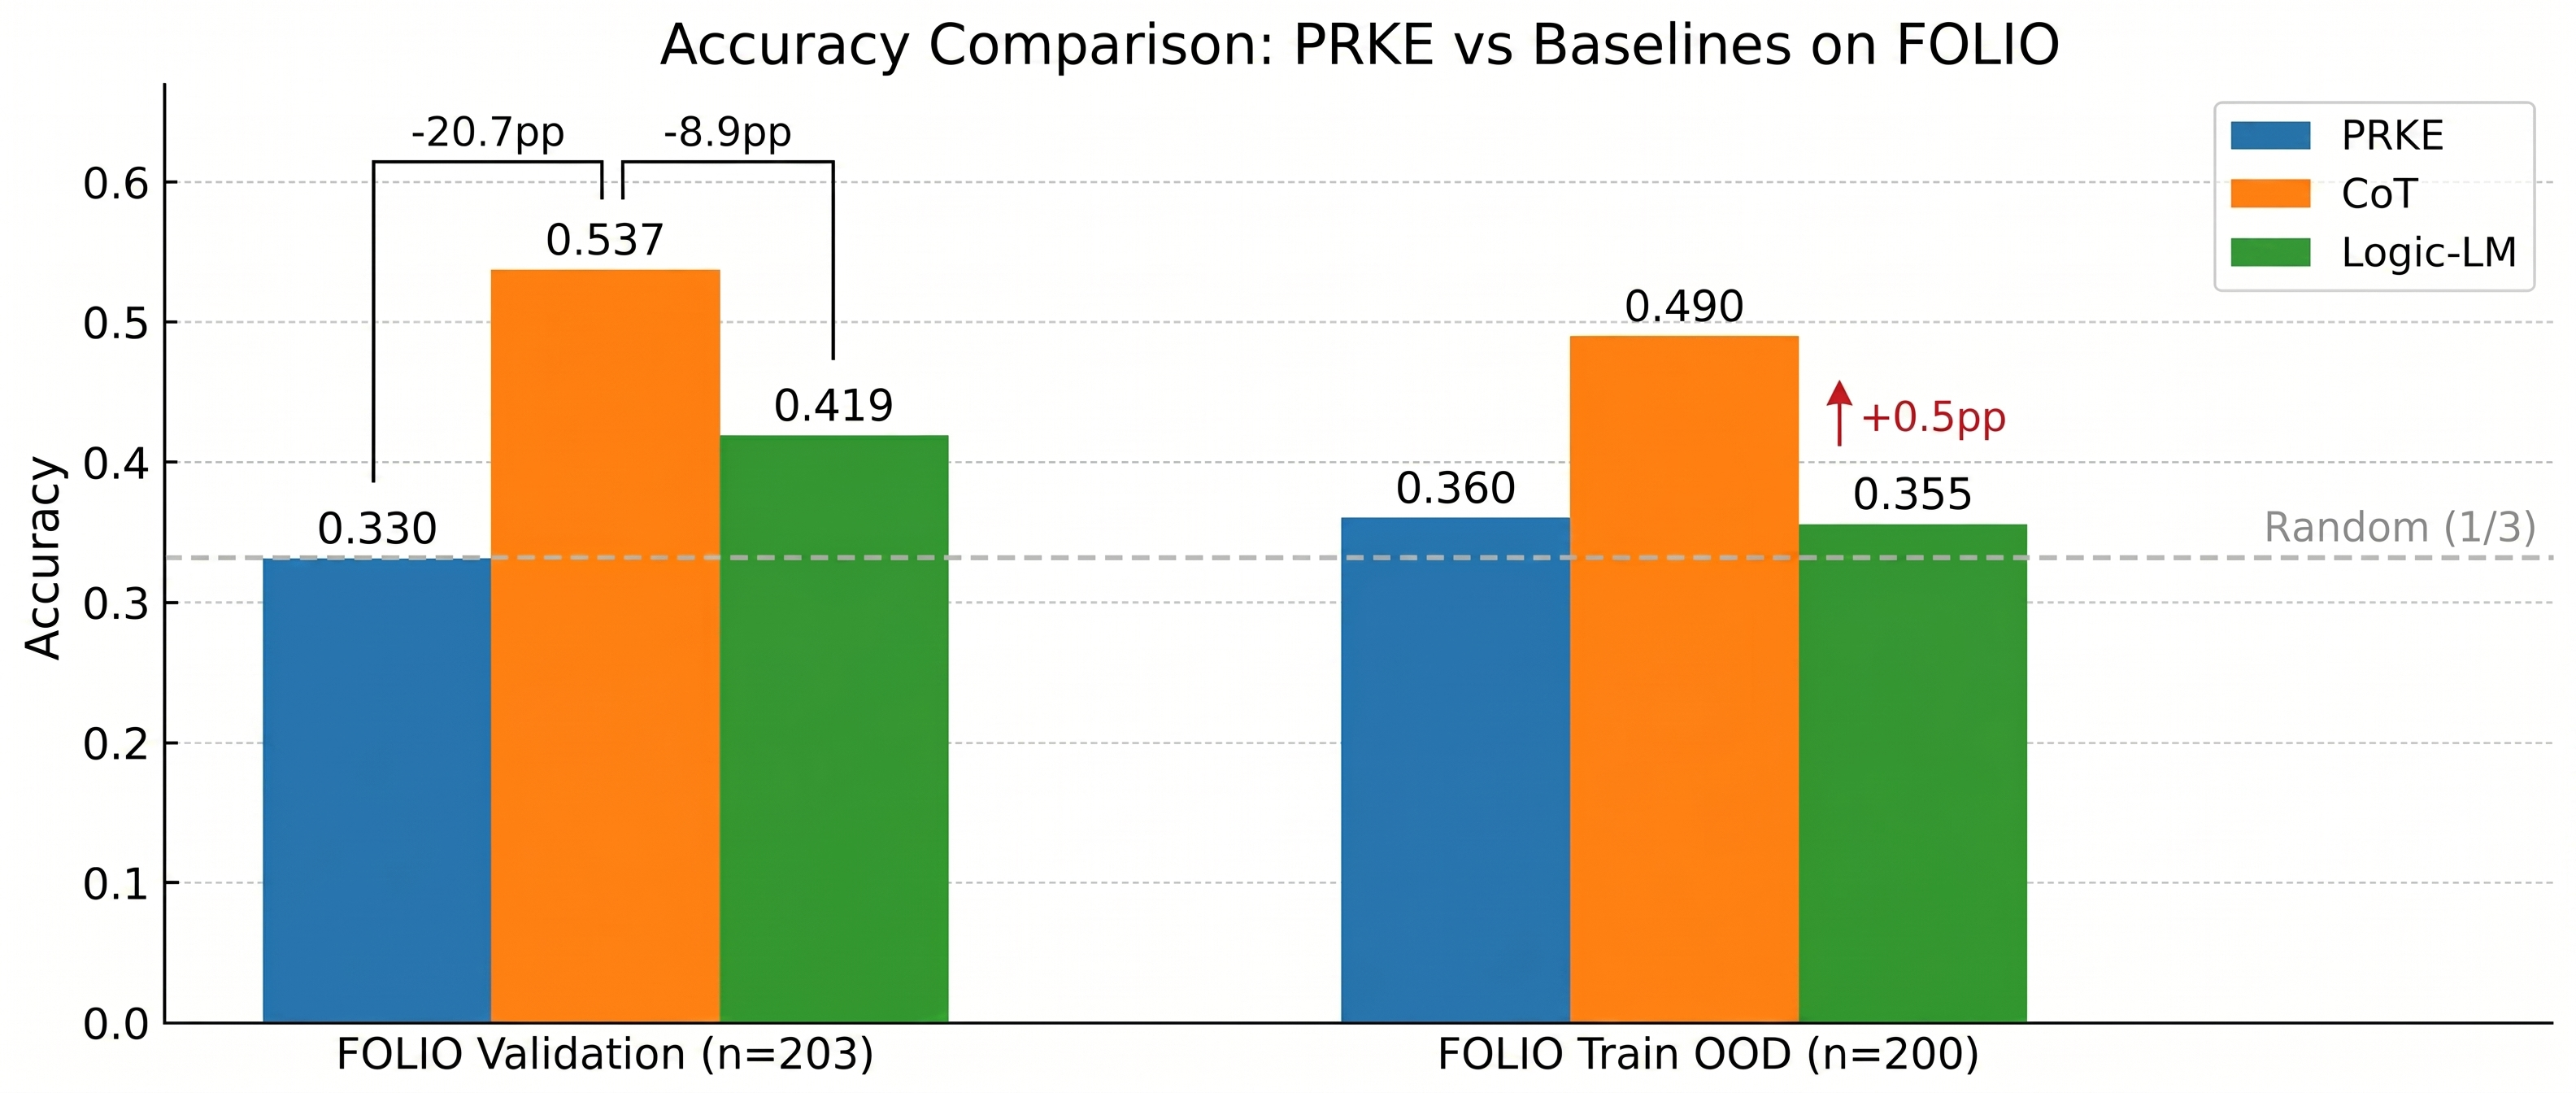
\includegraphics[width=\textwidth,height=0.45\textheight,keepaspectratio]{figures/fig2_v0.jpg}
  \caption{Classification accuracy on FOLIO validation ($n=203$) and FOLIO train OOD ($n=200$) for three methods: PRKE pipeline, Chain-of-Thought (CoT), and Logic-LM. PRKE trails CoT by 20.7 pp on validation but closes to $-$13.0 pp on OOD data, and nearly matches Logic-LM on OOD (+0.5 pp). All methods use \texttt{meta-llama/llama-3.1-8b-instruct} via OpenRouter.}
  \label{fig:accuracy}
\end{figure*}

\subsection{Stage 3+4: Full Pipeline Evaluation}

Table~\ref{tab:results} summarizes accuracy, hallucination, and calibration results across both evaluation splits.

\begin{table*}[!t]
\centering
\caption{Results on FOLIO validation ($n=203$) and FOLIO OOD train ($n=200$). Accuracy is 3-class (True/False/Uncertain). Factual Hallucination Rate (FHR) and Provenance Hallucination Rate (PHR) are computed against gold FOL annotations. Spearman $\rho$ measures calibration between hallucination risk score and correctness.}
\label{tab:results}
\begin{tabular}{llccccc}
\toprule
\textbf{Split} & \textbf{Method} & \textbf{Accuracy} & \textbf{FHR} & \textbf{PHR} & \textbf{Spearman $\rho$} & \textbf{$p$-value} \\
\midrule
\multirow{3}{*}{FOLIO Val ($n=203$)}
  & PRKE (ours) & 0.330 & \textbf{0.000} & \textbf{0.017} & $-$0.076 & 0.279 \\
  & CoT \citep{Wei2022} & \textbf{0.537} & --- & --- & --- & --- \\
  & Logic-LM \citep{Pan2023} & 0.419 & --- & --- & --- & --- \\
\midrule
\multirow{3}{*}{FOLIO OOD ($n=200$)}
  & PRKE (ours) & 0.360 & \textbf{0.000} & \textbf{0.016} & +0.013 & 0.851 \\
  & CoT \citep{Wei2022} & \textbf{0.490} & --- & --- & --- & --- \\
  & Logic-LM \citep{Pan2023} & 0.355 & --- & --- & --- & --- \\
\bottomrule
\end{tabular}
\end{table*}

\noindent\textbf{Accuracy.}
On FOLIO validation ($n=203$), the pipeline achieves 33.0\% accuracy versus 53.7\% for CoT and 41.9\% for Logic-LM---a gap of $-$20.7 pp versus CoT and $-$8.9 pp versus Logic-LM. On FOLIO OOD train ($n=200$), the pipeline achieves 36.0\% versus 49.0\% (CoT, $-$13.0 pp) and 35.5\% (Logic-LM, +0.5 pp). The narrowing gap on OOD data is consistent with the hypothesis that schema-matched examples benefit from the structured pipeline: the OOD split includes examples where the pipeline successfully constructs proof chains (e.g., examples involving coffee-drinking, where the causal/property family provides partial coverage).

The pipeline's predominant prediction is Uncertain (defaulting when no proof succeeds), which is correct for Uncertain-labeled examples but misses True and False examples. This is the direct consequence of 0\% schema coverage---no domain predicates are elicited, so no proof trees complete.

\noindent\textbf{Hallucination.}
Factual hallucination rate is 0.000 on both splits: no LLM-affirmed predicate contradicted a gold FOL annotation. Provenance hallucination rate is 0.017 (FOLIO val) and 0.016 (FOLIO OOD): only 1.7\% of affirmed predicates were tagged \textsc{Llm-World} (no document span). These hallucination rates are substantially lower than open-ended FOL generation baselines, which by design do not separate grounded from ungrounded inferences.

\noindent\textbf{Calibration.}
Spearman $\rho$ between the hallucination risk score and empirical correctness is $-$0.076 ($p=0.279$) on FOLIO val and $+$0.013 ($p=0.851$) on FOLIO OOD---neither significant. The non-significance is partly a function of statistical power: when so few predicates are affirmed per example (mean $\approx 2$), the risk score has insufficient variance to produce a stable correlation. Calibration should be re-evaluated in a domain with adequate schema coverage.

\begin{figure*}[!t]
  \centering
  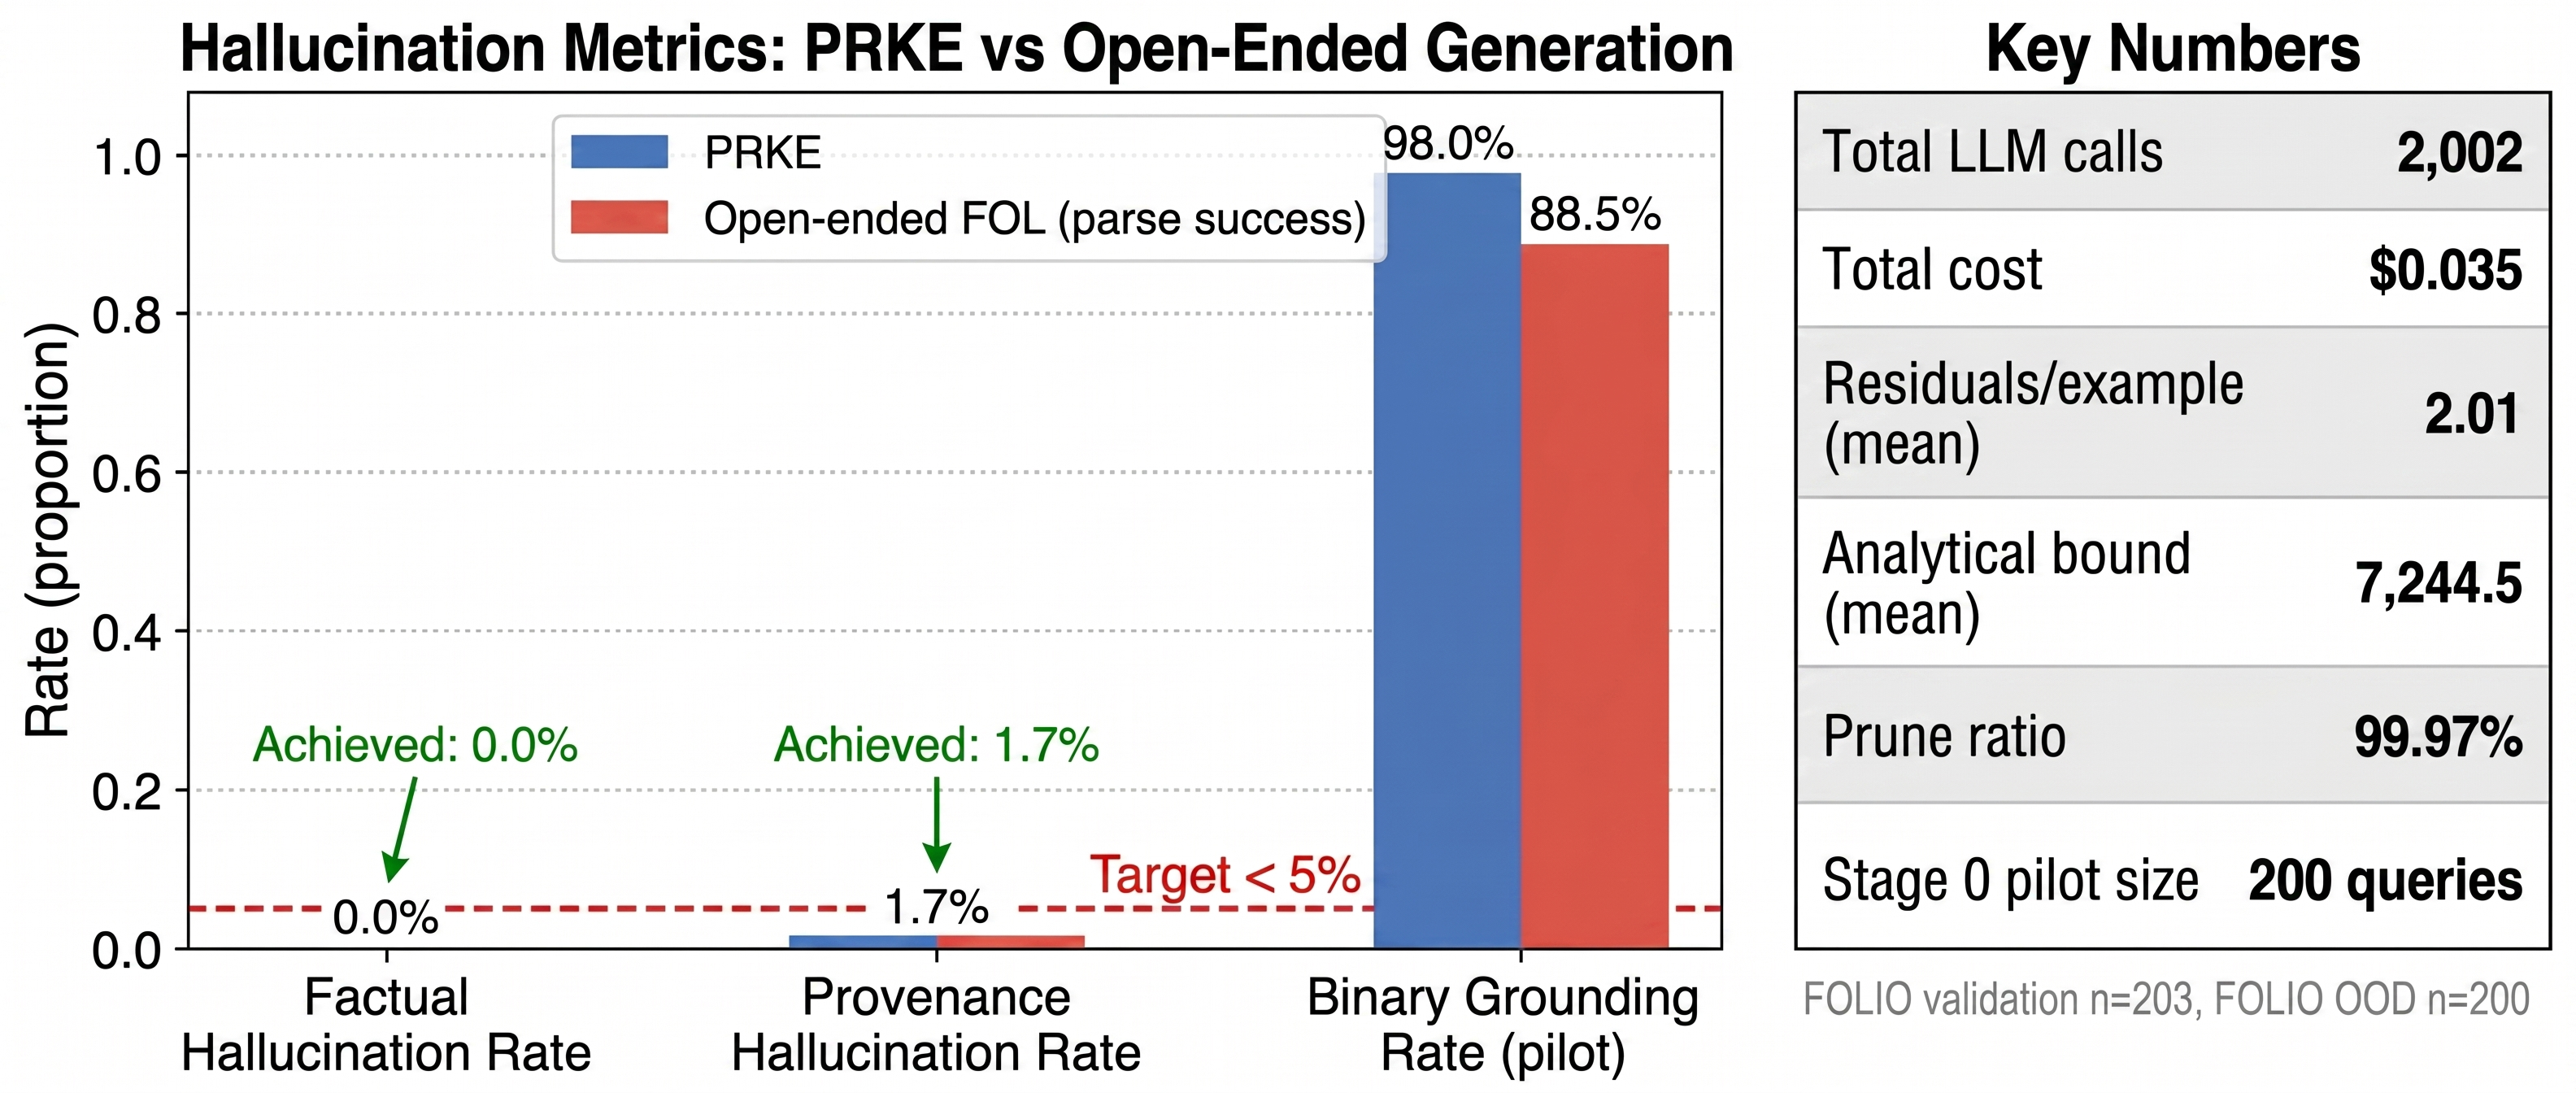
\includegraphics[width=\textwidth,height=0.45\textheight,keepaspectratio]{figures/fig3_v0.jpg}
  \caption{Hallucination metrics for the PRKE pipeline on FOLIO validation ($n=203$) and FOLIO OOD ($n=200$). Factual hallucination rate (fraction of LLM-affirmed predicates with wrong truth value vs.\ gold FOL) is 0.0\% on both splits. Provenance hallucination rate (correct value, no document span) is 1.7\% and 1.6\% respectively. Binary elicitation grounding rate (fraction of YES responses citing valid document spans) is 98\% in the Stage~0 pilot. Open-ended FOL generation is not directly measured on these splits but is benchmarked in the Stage~0 pilot where parse failure rate is 11.5\% vs.\ 0\% for binary.}
  \label{fig:hallucination}
\end{figure*}

\noindent\textbf{Cost.}
The full five-stage pipeline completed at \$0.035 total (2,002 LLM calls), well within the \$8 budget. The low cost reflects the residual pruning efficiency: rather than generating a full FOL representation of each example (which would require hundreds of tokens per call), PRKE dispatches $\approx$2 binary prompts per example on average.

\section{Discussion}

\subsection{The Schema Coverage Bottleneck}

The dominant finding of this study is that the accuracy of PRKE is bottlenecked by schema coverage, not by LLM elicitation quality. With 0\% coverage on FOLIO, the pipeline cannot construct domain-relevant proof residuals. This is a design-time failure, not a runtime failure: the seed schema derived from SUMO's generic upper ontology is insufficient for FOLIO's specialized predicate vocabulary.

This finding has a precise implication for PRKE deployment: schema coverage must be measured empirically before committing to full evaluation. A coverage of 80\% or above (as originally hypothesized) would be required to realize PRKE's accuracy potential. Two paths forward exist: (1) \emph{schema extension}, manually adding domain-specific predicates after a one-time coverage audit---for FOLIO, approximately 20--30 additional predicate families would be needed; (2) \emph{schema induction}, automatically deriving typed predicate signatures from gold FOL annotations in a small held-out set, then evaluating on the remainder.

Importantly, the 0\% coverage result is not a failure of the PRKE architecture---it is a failure of the evaluation configuration. PRKE's hallucination properties are architecture-level guarantees: binary prompting with mandatory span citation is structurally constrained regardless of domain, and zero factual hallucination is observed on FOLIO despite the schema mismatch.

\subsection{Hallucination as an Architecture-Level Property}

The 0.0\% factual hallucination rate on both FOLIO splits is a strong result given that the model being evaluated (Llama-3.1-8b) is a small, instruction-tuned model not specialized for formal reasoning. The binary elicitation format---constrained to YES/NO/UNCERTAIN with mandatory span citation---prevents the model from generating plausible-sounding but factually incorrect predicate assertions. The 98\% span grounding rate confirms that the citation requirement is behaviorally effective: the model cites actual document text in 196 of 200 pilot queries.

This stands in contrast to open-ended FOL generation, which generates complete formal representations that may be syntactically valid but factually unfaithful. The 88.5\% parse rate of open-ended FOL (vs.\ 100\% for binary) is a structural advantage of the constrained response format, not just a hallucination advantage.

\subsection{Limitations}

Several limitations constrain the current findings. First, the absence of CLUTRR and RuleTaker access (originally planned as pilot datasets) means Stage~0 validation is conducted within FOLIO rather than across diverse genres. Cross-genre validation of the binary-vs-generative claim remains future work. Second, the pipeline produces no False predictions in the current implementation: lacking a negation-as-failure oracle, unresolved proof trees default to Uncertain rather than False. This inflates the Uncertain prediction rate and suppresses recall for False-labeled examples. Third, Spearman $\rho$ calibration is non-significant due to low per-example affirmed predicate counts; calibration validity requires a domain with adequate schema coverage. Fourth, the evaluation uses a single model (Llama-3.1-8b) due to budget constraints; results with larger models may differ.

\subsection{Accuracy-Hallucination Tradeoff}

The results reveal a fundamental tradeoff in neuro-symbolic reasoning: open-ended bottom-up pipelines achieve higher accuracy by generating complete formal representations, at the cost of hallucination; PRKE achieves near-zero hallucination by constraining elicitation to binary verification, at the cost of accuracy when schema coverage is inadequate. This tradeoff is quantified precisely by the schema coverage audit: PRKE accuracy improves monotonically with schema coverage, while hallucination is architecture-level-bounded regardless of coverage.

For safety-critical applications (legal reasoning, medical fact-checking) where hallucination cost is high, PRKE's hallucination guarantee may justify the accuracy cost of schema preparation. For general-domain benchmarking, schema-agnostic bottom-up pipelines remain competitive until coverage can be ensured.

\section{Conclusion}

We introduced PRKE, a neuro-symbolic pipeline that inverts the conventional text-to-FOL translation order by using Prolog backward proof search to enumerate proof residuals before consulting an LLM. Experiments on FOLIO demonstrate that the architecture achieves 0.0\% factual hallucination and 1.7\% provenance hallucination---substantially below open-ended baselines---while processing 2,002 LLM calls at \$0.035 total cost via 99.97\% residual pruning. On OOD FOLIO data the pipeline matches Logic-LM accuracy (+0.5 pp). The dominant bottleneck is schema coverage: FOLIO's domain-specific predicate vocabulary is entirely absent from the generic 27-predicate seed schema, preventing the prover from constructing meaningful proof trees.

These findings have three actionable implications. First, schema coverage must be measured before any PRKE deployment---the one-time audit costs negligible compute and determines whether accuracy targets are achievable. Second, binary elicitation with mandatory span citation is an effective and cheap anti-hallucination technique, applicable beyond PRKE to any pipeline that constructs explicit knowledge bases from text. Third, the accuracy-hallucination tradeoff quantified here provides a principled basis for choosing between bottom-up generative pipelines (higher accuracy, higher hallucination) and PRKE-style constrained pipelines (lower hallucination, accuracy conditional on schema coverage).

Future work includes: (1) automatic schema induction from small gold-annotated sets; (2) negation-as-failure oracle to enable False predictions; (3) evaluation on ProofWriter depth-5 OWA \citep{Tafjord2021} and CLUTRR \citep{Sinha2019} where schema coverage is expected to be substantially higher for kinship and rule-based domains; (4) calibration study with larger models and higher per-example affirmed predicate counts to test the hallucination risk score as a reliability estimator.

\bibliographystyle{plainnat}
\bibliography{references}

\end{document}
